%% 
%% Copyright 2007, 2008, 2009 Elsevier Ltd
%% 
%% This file is part of the 'Elsarticle Bundle'.
%% ---------------------------------------------
%% 
%% It may be distributed under the conditions of the LaTeX Project Public
%% License, either version 1.2 of this license or (at your option) any
%% later version.  The latest version of this license is in
%%    http://www.latex-project.org/lppl.txt
%% and version 1.2 or later is part of all distributions of LaTeX
%% version 1999/12/01 or later.
%% 
%% The list of all files belonging to the 'Elsarticle Bundle' is
%% given in the file `manifest.txt'.
%% 

%% Template article for Elsevier's document class `elsarticle'
%% with numbered style bibliographic references
%% SP 2008/03/01

\documentclass[preprint,12pt, a4paper]{elsarticle}

%% Use the option review to obtain double line spacing
%% \documentclass[authoryear,preprint,review,12pt]{elsarticle}

%% For including figures, graphicx.sty has been loaded in
%% elsarticle.cls. If you prefer to use the old commands
%% please give \usepackage{epsfig}

%% The amssymb package provides various useful mathematical symbols
\usepackage{amssymb}
\usepackage{color}
\usepackage{hyperref}
\setlength{\parindent}{0pt}
%% The amsthm package provides extended theorem environments
%% \usepackage{amsthm}

%% The lineno packages adds line numbers. Start line numbering with
%% \begin{linenumbers}, end it with \end{linenumbers}. Or switch it on
%% for the whole article with \linenumbers.
%\usepackage{lineno}

\journal{SoftwareX}

\begin{document}
\renewcommand{\labelenumii}{\arabic{enumi}.\arabic{enumii}}

\begin{frontmatter}

%% Title, authors and addresses

%% use the tnoteref command within \title for footnotes;
%% use the tnotetext command for the associated footnote;
%% use the fnref command within \author or \address for footnotes;
%% use the fntext command for the associated footnote;
%% use the corref command within \author for corresponding author footnotes;
%% use the cortext command for the associated footnote;
%% use the ead command for the email address,
%% and the form \ead[url] for the home page:
%% \title{Title\tnoteref{label1}}
%% \tnotetext[label1]{}
%% \author{Name\corref{cor1}\fnref{label2}}
%% \ead{email address}
%% \ead[url]{home page}
%% \fntext[label2]{}
%% \cortext[cor1]{}
%% \address{Address\fnref{label3}}
%% \fntext[label3]{}

\title{gamma\_flow: \textbf{G}uided \textbf{A}nalysis of \textbf{M}ulti-label spectra by \textbf{Ma}trix \textbf{F}actorization for \textbf{L}ightweight \textbf{O}perational \textbf{W}orkflows}

%% use optional labels to link authors explicitly to addresses:
%% \author[label1,label2]{}
%% \address[label1]{}
%% \address[label2]{}

\author[ki-lab]{Viola Rädle \corref{cor1}}
\author[ki-lab]{Tilman Hartwig}
\author[ki-lab]{Benjamin Oesen}
\author[bfs]{Emily Alice Kröger}
\author[bfs]{Julius Vogt}
\author[bfs]{Eike Gericke}
\author[bfs]{Martin Baron}

\address[ki-lab]{Application Lab for AI and Big Data, German Environmental Agency, Leipzig, Germany}
\address[bfs]{Federal Office for Radiation Protection, Berlin, Germany}

\cortext[cor1]{Corresponding author: raedle.htwk@web.de}


\begin{abstract}
\textcolor{blue}{
\textbf{gamma\_flow} is an open-source Python package for real-time analysis of spectral data. It supports classification, denoising, decomposition, and outlier detection of both single- and multi-component spectra. Instead of relying on large, computationally intensive models, it employs a novel supervised approach to non-negative matrix factorization (NMF) for dimensionality reduction. This ensures a fast, efficient, and adaptable analysis while reducing computational costs. \textbf{gamma\_flow} achieves classification accuracies above 90\% and enables reliable automated spectral interpretation. Originally developed for gamma-ray spectra, it is applicable to any type of one-dimensional spectral data. As an open and flexible alternative to proprietary software, it supports various applications in research and industry.} 
\end{abstract}

\begin{keyword}
Python \sep Gamma spectroscopy \sep Non-negative Matrix Factorization \sep Classification \sep Denoising \sep Spectral Deconvolution

%% PACS codes here, in the form: \PACS code \sep code

%% MSC codes here, in the form: \MSC code \sep code
%% or \MSC[2008] code \sep code (2000 is the default)

\end{keyword}

\end{frontmatter}

%\linenumbers

\section*{Metadata}
\label{}
\textit{The ancillary data table~\ref{codeMetadata} is required for the sub-version of the codebase. Please replace the italicized text in the right column with the correct information about your current code and leave the left column untouched.}

\begin{table}[!h]
\begin{tabular}{|l|p{6.5cm}|p{6.5cm}|}
\hline
\textbf{Nr.} & \textbf{Code metadata description} & \textbf{Metadata} \\
\hline
TO DO C1 & Current code version & For example v42 \\
\hline
C2 & Permanent link to code/repository used for this code version & \url{https://gitlab.opencode.de/uba-ki-lab/gamma_flow} \\
\hline
C3  & Permanent link to Reproducible Capsule & TO DO For example: \url{https://codeocean.com/capsule/0270963/tree/v1}\\
\hline
C4 & Legal Code License   & BSD 3-Clause "New" or "Revised" License \\
\hline
C5 & Code versioning system used & git\\
\hline
C6 & Software code languages, tools, and services used & Python \\
\hline
C7 & Compilation requirements, operating environments \& dependencies & TO DO. Jupyter?  \\
\hline
C8 & If available Link to developer documentation/manual & \url{https://gitlab.opencode.de/uba-ki-lab/gamma_flow/-/blob/main/README.md?ref_type=heads} \\
\hline
C9 & Support email for questions & raedle.htwk@web.de\\
\hline
\end{tabular}
\caption{Code metadata (mandatory)}
\label{codeMetadata} 
\end{table}

\textcolor{red}{\textit{Optionally, you can provide information about the current executable
software version filling in the left column of
Table~\ref{executabelMetadata}. Please leave the first column as it is.} FRAGE: Welche Tabelle sollen wir ausfüllen?}

\begin{table}[!h]
\begin{tabular}{|l|p{6.5cm}|p{6.5cm}|}
\hline
\textbf{Nr.} & \textbf{(Executable) software metadata description} & \textbf{Please fill in this column} \\
\hline
S1 & Current software version & For example 1.1, 2.4 etc. \\
\hline
S2 & Permanent link to executables of this version  & For example: \url{https://github.com/combogenomics/DuctApe/releases/tag/DuctApe-0.16.4} \\
\hline
S3  & Permanent link to Reproducible Capsule & \\
\hline
S4 & Legal Software License & List one of the approved licenses \\
\hline
S5 & Computing platforms/Operating Systems & For example Android, BSD, iOS, Linux, OS X, Microsoft Windows, Unix-like , IBM z/OS, distributed/web based etc. \\
\hline
S6 & Installation requirements \& dependencies & \\
\hline
S7 & If available, link to user manual - if formally published include a reference to the publication in the reference list & For example: \url{http://mozart.github.io/documentation/} \\
\hline
S8 & Support email for questions & \\
\hline
\end{tabular}
\caption{Software metadata (optional)}
\label{executabelMetadata} 
\end{table}


\section{Motivation and significance}
\textit{In this section, we want you to introduce the scientific background and the motivation for developing the software.}

\begin{itemize}
    \item \textit{Explain why the software is important and describe the exact (scientific) problem(s) it solves.}
    \item \textit{Indicate in what way the software has contributed (or will contribute in the future) to the process of scientific discovery; if available, please cite a research paper using the software.}
    \item \textit{Provide a description of the experimental setting. (How does the user use the software?)}
    \item \textit{Introduce related work in literature (cite or list algorithms used, other software etc.).}
\end{itemize}

Most radioactive sources can be identified by measuring their emitted radiation (X-rays and gamma rays), and visualizing them as a spectrum. In nuclear security applications, the resulting gamma spectra have to be analyzed in real-time as immediate reaction and decision making may be required. 
However, the manual recognition of isotopes present in a spectrum constitutes a 
strenous, error-prone task that depends upon expert knowledge. Hence, this raises 
the need for algorithms assisting in the initial categorization and recognizability 
of measured gamma spectra. 
The delineated use case brings along several requirements:  
\begin{itemize}
\item As mobile, room temperature detectors are often deployed in nuclear security applications, the produced spectra typically exhibit a rather low energy resolution. In addition, a high temporal resolution is required (usually around one spectrum per second), leading to a low acquisition time and a low signal-to-noise ratio. Hence, the model must be robust and be able to handle noisy data.  
\item For some radioactive sources, acquisition of training spectra may be challenging. Instead, spectra of those isotopes are simulated using Monte Carlo N-Particle (MCNP) code \cite{Kulesza2022}. In this process, energy deposition in a detector material is simulated, yielding spectra that can be used for model training. However, simulated spectra and measured spectra from real-world sources may differ, which may be a constraint for model performance. On this account, preliminary data exploration is crucial to assess the similarity of spectral data from different detectors and to evaluate potential data limitations.  
\item Lastly, not only the correct classification of single-label test spectra (stemming from one isotope) is necessary, but also the decomposition of linear combinations of various isotopes (multi-label spectra). Hence, classification approaches like k-nearest-neighbours that solely depend on the similarity between training and test spectra are not applicable.  
\end{itemize} 
This paper presents \textbf{gamma\_flow}, a Python package designed for the real-time analysis of one-dimensional spectra. It was developed in response to the practical challenges described above and supports the following tasks:
\begin{itemize}
\item classification of test spectra to identify their constituents,  
\item denoising to enhence visibility and reduce measurement noise,
\item outlier detection to evaluate the model's applicability to test spectra.   
\end{itemize}

Originally developed for gamma spectroscopy, \textbf{gamma\_flow} is applicable to various domains including material science, chemistry, and environmental monitoring. It facilitates automated analysis in settings where fast interpretation of spectral data is essential. By integrating supervised dimensionality reduction with classical signal processing techniques, it extends prior work such as that of Bilton et al. \cite{Bilton2019}, contributing to reproducible and interpretable spectral analysis pipelines.



\section{Software description}

\textit{Describe the software. Provide enough detail to help the reader understand its impact. }
\textcolor{blue}{
\textbf{gamma\_flow} is based on a dimensionality reduction model that constitutes a novel, supervised approach to non-negative matrix factorization (NMF). More explicitly, the spectral data matrix is decomposed into the product of two low-rank matrices denoted as the scores (spectral data in latent space) and the loadings (transformation matrix or latent components). The loadings matrix is predefined and consists of the mean spectra of the training isotopes. Hence, by design, the scores axes correspond to the share of an isotope in a spectrum, resulting in an interpretable latent space. 
As a result, the classification of a test spectrum can be read directly from its (normalized) 
scores. In particular, shares of individual isotopes in a multi-label spectrum can be 
identified. This leads to an explainable quantitative prediction of the spectral constituents. 
The scores can be transformed back into spectral space by applying the inverse model. This 
inverse transformation rids the test spectrum of noise and results in a smooth, easily 
recognizable denoised spectrum. 
If a test spectrum of an isotope is unknown to the model (i.e. this isotope was not included in 
model training), it can still be projected into latent space. However, when the latent space 
information (scores) are decompressed, the resulting denoised spectrum does not resemble the 
original spectrum any more. Some original features may not be captured while new peaks may have 
been fabricated. This can be quantified by calculating the cosine similarity between the original and the denoised spectrum, which can serve as an indicator of a test spectrum 
to be an outlier.}

\subsection{Software architecture}
\textit{  Give a short overview of the overall software architecture; provide a pictorial overview where possible; for example, an image showing the components. If necessary, provide implementation details.}
\textcolor{red}{Soll hier ein Schaubild erstellt werden von jupyter-files und auf welche python-files sie zugreifen? To do: Jore fragen, automatisches Schaubild erstellen in VSCode? Pycallgraph, mermaid,...}

 \subsection{Software functionalities}
\textit{Present the major functionalities of the software.}

This python package consists of three jupyter notebooks that are executed consecutively. 
In this section, their functionality and is outlined, with an emphasis on the mathematical 
structure of the model. 

\subsubsection{Preprocessing and data exploration}  
The notebook \texttt{01\_preprocessing.ipynb} synchronizes spectral data and provides a framework 
of visualizations for data exploration. All functions called in this notebook are found 
in \texttt{tools\_preprocessing.py}. 

During \textbf{preprocessing}, the following steps are performed:   
\begin{itemize}
\item Spectral data files are converted from .xlsm/.spe data to .npy format and saved.  
\item Spectra of different energy calibrations are rebinned to a standard energy calibration.  
\item Spectral data are aggregated by label classes and detectors. Thus, it is possible to 
  collect data from different files and formats.  
\item Optional: The spectra per isotope are limited to a maximum number.  
\item The preprocessed spectra are saved as .npy files.  
\end{itemize}


\textbf{Data exploration} involves the following visualizations: 
\begin{itemize}
\item For each label class (e.g. for each isotope), the mean spectra are calculated detector-wise and compared 
  quantitatively by the cosine similarity.  
\item For each label class, example spectra are chosen randomly and plotted to provide an overview
  over the data.  
\item The cosine similarity is calculated and visualized as a matrix for all label classes and detectors. 
\end{itemize}
This helps to assess whether the model can handle spectra from different detectors.   


\subsubsection{Model training and testing}
The notebook \texttt{02\_model.ipynb} trains and tests a dimensionality reduction model that allows for denoising, classification and outlier detection of test spectra. All functions called in this notebook are found in \texttt{tools\_model.py}.

The dimensionality reduction model presented in this paper comprises a matrix decomposition of spectral data. More precisely, the original spectra matrix $X$ is reconstructed by two low-rank matrices $S$ and $L$:  
$$ X \approx S  L^{T} $$  
with $S$: scores matrix (spectra in latent space) \\  
\hspace*{0.8cm} $L$: loadings matrix (transformation matrix or latent components). \\ 

\begin{figure}
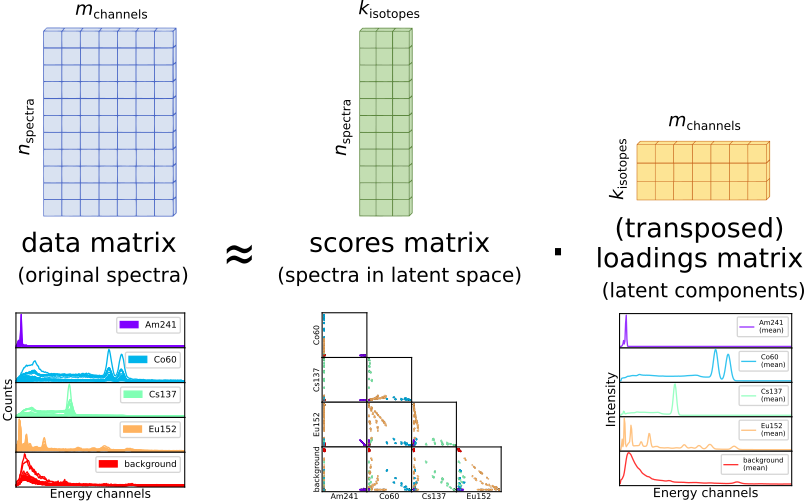
\includegraphics[width=\textwidth]{figure_1.png}
\label{fig:matrix_decomposition}
\end{figure}

As illustrated in Figure \ref{fig:matrix_decomposition}, original spectral data can be compressed into $k_\mathrm{isotopes}$ dimensions. To ensure a conclusive assignment of the latent space axes to the isotopes (i.e. one axis stands for of one isotope), the loadings matrix is predefined as the mean spectra of the $k_\mathrm{isotopes}$ isotopes. 

During model training, mean spectra for all isotopes are calculated. The scores are then derived by non-negative least squares fit of the original spectra to the loadings matrix. Thus, the components of the normalized scores vectors directly reveal the contributions of the individual isotopes. Denoised spectra, on the other hand, are computed by transforming the non-normalized scores back into spectral space (i.e. by multiplication of with the loadings matrix).

In mathematical terms, this model represents a 'supervised' approach to Non-negative Matrix Factorization (NMF) \cite{Shreeves2020, Bilton2019}. 
While dimensionality reduction is conventionally an unsupervised task as it 
only considers data structure \cite{Olaya2022}, our approach integrates labels in model training. This leads to an interpretable latent space and obviates the need for an additional classification step. While other supervised NMF approaches incorporate classification loss in model training \cite{Leuschner2019, Lee2010, Bisot2016}, our model focuses on a comprehensible construction of the latent space. 


The model is trained using spectral data from the specified detectors \texttt{dets\_tr} and isotopes \texttt{isotopes\_tr}. Subsequently, it is inferenced (i.e. scores are calculated) on three different test datasets:
\begin{enumerate}
\item validation data/holdout data from same detector as used in training (each spectrum including 
only one isotope or pure background)
\item test data from different detector (each spectrum including one isotope and background)
\item multi-label test data from different detector (each spectrum including multiple isotopes and background)
\end{enumerate}


For all test datasets, spectra are classified and denoised. The results are visualized as 
\begin{itemize}
\item confusion matrix  
\item misclassified spectra  
\item denoised example spectrum  
\item misclassification statistics  
\item scores as scatter matrix  
\item mean scores as bar plot
\end{itemize}
  
This helps to assess model performance with respect to classification and denoising. 

\subsubsection{Outlier analysis}
The notebook \texttt{03\_outlier.ipynb} provides an exploratory approach to outliers detection, i.e. to identify spectra from isotopes that were not used in model training. All functions called in this notebook are found in \texttt{tools\_outlier.py}. 

To simulate outlier spectra, a mock dataset is generated by training a model after removing one specific isotope. The trained model is then inferenced on spectra of this unknown isotope to investigate its behaviour with outliers. 
First, the resulting latent space distribution and further meta data are analyzed to distinguish known from unknown spectra. Using a decision tree, the most informative feature is identified. 
Next, a decision boundary is derived for this feature, by  \\
a) using the condition of the first split in the decision tree \\
b) fitting a logistic regression (sigmoid function) to the data \\ 
c) setting a manual threshold by considering accuracy, precision and recall of outlier identification. \\
The derived decision boundary can then be implemented in the measurement pipeline by the user. \\


Apart from the jupyter notebooks and python files described above, the project includes the following python files:  
\begin{itemize}
\item \texttt{globals.py}: global variables  
\item \texttt{plotting.py}: all visualizations and plotting routines    
\item \texttt{util.py}: basic functions that are used by all notebooks  
\end{itemize}

  
\subsection{Sample code snippets analysis (optional)}
\textcolor{red}{Würde ich eher weglassen? Ggf. Das Modell vorstellen, aber eher nicht}

\section{Illustrative examples}

\textit{Provide at least one illustrative example to demonstrate the major
functions of your software/code.}

\textit{\textbf{Optional}: you may include one explanatory  video or screencast that will appear next to your article, in the right hand side panel. Please upload any video as a single supplementary file with your article. Only one MP4 formatted, with 150MB maximum size, video is possible per article. Recommended video dimensions are 640 x 480 at a maximum of 30 frames / second. Prior to submission please test and validate your .mp4 file at  \url{http://elsevier-apps.sciverse.com/GadgetVideoPodcastPlayerWeb/verification} . This tool will display your video exactly in the same way as it will appear on ScienceDirect. }

\textcolor{blue}{
Plots: 
\begin{itemize}
	\item Confusion matrix (different detector, single-label class.)
	\item Denoised spectrum
	\item ggf. Outlier: Feature importance (decision tree)
\end{itemize}}


\section{Impact}
\textit{This is the main section of the article and reviewers will weight it appropriately.
Please indicate:}
\begin{itemize}
    \item \textit{Any new research questions that can be pursued as a result of your software.}
    \item \textit{In what way, and to what extent, your software improves the pursuit of existing research questions.}
    \item \textit{Any ways in which your software has changed the daily practice of its users.}
    \item \textit{How widespread the use of the software is within and outside the intended user group (downloads, number of users if your software is a service, citable publications, etc.).}
    \item \textit{How the software is being used in commercial settings and/or how it has led to the creation of spin-off companies.}
    \end{itemize}
\textit{Please note that points 1 and 2 are best demonstrated by
  references to citable publications.}

\textcolor{blue}{\textbf{übernommen aus JOSS-Statement of need}:
In many research fields, spectral measurements help to assess material properties. 
In this context, an area of interest for many researchers is the classification (automated 
labelling) of the measured spectra. Proprietary spectral analysis software, however, are often 
limited in their functionality and adaptability \cite{Lam2011, Nasereddin2023}. 
In addition, the underlying mechanisms are usually not revealed and may act as a black-box 
system to the user \cite{ElAmri2022}. On top of that, a spectral comparison is typically only possible for spectra of pure substances \cite{Cowger2021}. However, there may be a need to decompound multi-label spectra (linear combinations of different substances) and identify their constituents. \newline
\textbf{gamma\_flow} is a Python package that can assist researchers in the classification,
denoising and outlier detection of spectra. It includes data preprocessing, 
data exploration, model training and testing as well as an exploratory section
on outlier detection. 
Making use of matrix decomposition methods, the designed model is lean and performant. 
Training and inference do not require special hardware or extensive computational
power. This allows real-time application on ordinary laboratory computers and 
easy implementation into the measurement routine. 
The provided example dataset contains gamma spectra of several measured and simulated 
isotopes as well as pure background spectra. 
While this package was developed in need of an analysis tool for gamma spectra, 
it is suitable for any one-dimensional spectra.  
Examplary applications encompass  
\begin{itemize}
\item \textbf{Infrared spectroscopy} for the assessment of the polymer composition of 
microplastics in water \cite{Ferreiro2023, Whiting2022}  
\item \textbf{mass spectrometry} for protein identification in snake venom 
\cite{Zelanis2019, Yasemin2021}  
\item \textbf{Raman spectroscopy} for analysis of complex pharmaceutical mixtures and detection
of dilution products like lactose \cite{Fu2021}  
\item \textbf{UV-Vis spectroscopy} for detection of pesticides in surface waters \cite{Guo2020, Qi2024}
\item \textbf{stellar spectroscopy} to infer the chemical composition of stars \cite{Gray2021}  
\end{itemize}
}



\section{Conclusions}
... to do

\section*{Acknowledgements}
\label{}
We gratefully acknowledge the support provided by the Federal Ministry for the Environment, Nature Conservation and Nuclear Safety (BMUV), whose funding has been instrumental in enabling us to achieve our research objectives and explore new directions. 
We also extend our appreciation to Martin Bussick in his function as the AI coordinator. 
Additionally, we thank the entire AI-Lab team for their support and inspiration, with special recognition to Ruth Brodte for guidance on legal and licensing matters.


%% The Appendices part is started with the command \appendix;
%% appendix sections are then done as normal sections
%% \appendix

%% \section{}
%% \label{}

%% References:
%% If you have bibdatabase file and want bibtex to generate the
%% bibitems, please use
%%
%%  \bibliographystyle{elsarticle-num} 
%%  \bibliography{<your bibdatabase>}

%% else use the following coding to input the bibitems directly in the
%% TeX file.
\bibliographystyle{elsarticle-num} 
\bibliography{gamma_flow_SoftwareX.bib}
\begin{thebibliography}{00}

%% \bibitem{label}
%% Text of bibliographic item

\bibitem{} Use this style of ordering. References in-text should also use a similar style.

\end{thebibliography}

\textit{If the software repository you used supplied a DOI or another
Persistent IDentifier (PID), please add a reference for your software
here. For more guidance on software citation, please see our guide for
authors or \href{https://f1000research.com/articles/9-1257/v2}{this
  article on the essentials of software citation by FORCE 11}, of
which Elsevier is a member.}

\large{\textbf{Reminder: Before you submit, please delete all 
the instructions in this document, 
including this paragraph. 
Thank you!}}




\end{document}
\endinput
%%
%% End of file `SoftwareX_article_template.tex'.

%%% Local Variables:
%%% mode: latex
%%% TeX-master: t
%%% End:
